% ----------------------------------------------------------------- %
%             The Speech Signal Processing Toolkit (SPTK)           %
%             developed by SPTK Working Group                       %
%             http://sp-tk.sourceforge.net/                         %
% ----------------------------------------------------------------- %
%                                                                   %
%  Copyright (c) 1984-2007  Tokyo Institute of Technology           %
%                           Interdisciplinary Graduate School of    %
%                           Science and Engineering                 %
%                                                                   %
%                1996-2010  Nagoya Institute of Technology          %
%                           Department of Computer Science          %
%                                                                   %
% All rights reserved.                                              %
%                                                                   %
% Redistribution and use in source and binary forms, with or        %
% without modification, are permitted provided that the following   %
% conditions are met:                                               %
%                                                                   %
% - Redistributions of source code must retain the above copyright  %
%   notice, this list of conditions and the following disclaimer.   %
% - Redistributions in binary form must reproduce the above         %
%   copyright notice, this list of conditions and the following     %
%   disclaimer in the documentation and/or other materials provided %
%   with the distribution.                                          %
% - Neither the name of the SPTK working group nor the names of its %
%   contributors may be used to endorse or promote products derived %
%   from this software without specific prior written permission.   %
%                                                                   %
% THIS SOFTWARE IS PROVIDED BY THE COPYRIGHT HOLDERS AND            %
% CONTRIBUTORS "AS IS" AND ANY EXPRESS OR IMPLIED WARRANTIES,       %
% INCLUDING, BUT NOT LIMITED TO, THE IMPLIED WARRANTIES OF          %
% MERCHANTABILITY AND FITNESS FOR A PARTICULAR PURPOSE ARE          %
% DISCLAIMED. IN NO EVENT SHALL THE COPYRIGHT OWNER OR CONTRIBUTORS %
% BE LIABLE FOR ANY DIRECT, INDIRECT, INCIDENTAL, SPECIAL,          %
% EXEMPLARY, OR CONSEQUENTIAL DAMAGES (INCLUDING, BUT NOT LIMITED   %
% TO, PROCUREMENT OF SUBSTITUTE GOODS OR SERVICES; LOSS OF USE,     %
% DATA, OR PROFITS; OR BUSINESS INTERRUPTION) HOWEVER CAUSED AND ON %
% ANY THEORY OF LIABILITY, WHETHER IN CONTRACT, STRICT LIABILITY,   %
% OR TORT (INCLUDING NEGLIGENCE OR OTHERWISE) ARISING IN ANY WAY    %
% OUT OF THE USE OF THIS SOFTWARE, EVEN IF ADVISED OF THE           %
% POSSIBILITY OF SUCH DAMAGE.                                       %
% ----------------------------------------------------------------- %
\hypertarget{fftr2}{}
\name{fftr2}{2-dimensional FFT for real sequence}{signal processing}

\begin{synopsis}
\item[fftr2] [ --l $L$ ] [ --m $M_1 \; M_2$ ] [ --t ] [ --c ] [ --q ] 
	     [ --\{ A $|$ R $|$ I $|$ P \} ] [ {\em infile} ] 
\end{synopsis}

\begin{qsection}{DESCRIPTION}
{\em fftr2} uses the 2-dimensional Fast Fourier Transform (FFT) algorithm 
to calculate the 2-dimensional Discrete Fourier Transform (DFT) 
of real-valued input data from {\em infile} (or standard input), 
sending the result to standard output. 
The input and output data is in float format, arranged as follows.
\begin{center}
 \leavevmode
 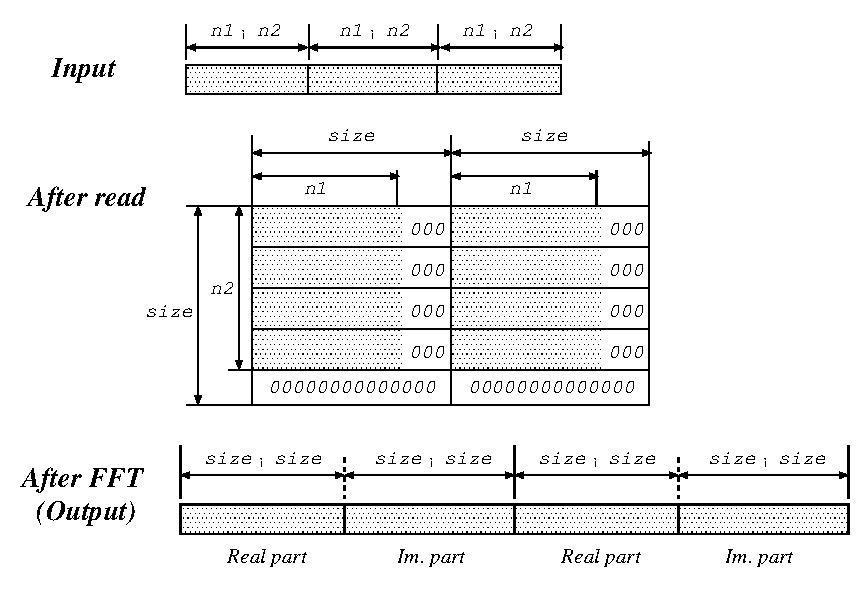
\includegraphics{fig/fftr2.eps}
\end{center}
\end{qsection}

\begin{options}
	\argm{l}{L}{FFT size  power of 2}{64}
	\argm{m}{M_1 \; M_2}{order of sequence ($M_1\times M_2$).
			If the file size $k$ is smaller than $64^2$
			and $\sqrt{k}$ is integer value, $M_1=M_2=\sqrt{k}$. 
			Otherwise output error message to standard error output 
			and then terminate.}{$64 , M_1$}
	\argm{t}{}{Output results in transposed form (see also \hyperlink{fft2}{fft2}).}{FALSE}
	\argm{c}{}{When results are transposed, 1 boundary data is copied from the
	opposite side, and then output $(L+1)\times (L+1)$ data (see also \hyperlink{fft2}{fft2}).}{FALSE}
	\argm{q}{}{Output first $1/4$ data of FFT results only.
		   As in the above c option, boundary data is compensated and 
		   $(\frac{L}{2}+1)\times(\frac{L}{2}+1)$ data are output
		   (see also \hyperlink{fft2}{fft2}).}{FALSE}
	\argm{A}{}{amplitude}{FALSE}
	\argm{R}{}{real part}{FALSE}
	\argm{I}{}{imaginary part}{FALSE}
	\argm{P}{}{output power spectrum}{FALSE}
\end{options}

\begin{qsection}{EXAMPLE}
This example reads a sequence of 2-dimensional real numbers in float format
from {\em data.f} file, evaluates its 2-dimensional DFT and outputs results to {\em
data.dft} file:
\begin{quote}
  \verb!fftr2 -A data.f > data.dft!
\end{quote}
\end{qsection}

\begin{qsection}{SEE ALSO}
\hyperlink{fft}{fft},
\hyperlink{fft2}{fft2},
\hyperlink{ifft}{ifft}
\end{qsection}
